\chapter{Propagation in a turbulent atmosphere}\label{chapter:turbulence}\todo{From paper. Rewrite}

\section{Introduction}

% TODO: rewrite paragraph from paper
In an outdoor situation, spatial and temporal variations in temperature and wind
velocity cause small changes in the refractive index. As waves pass through the
atmosphere, the index-of-refraction variations in effect cause scintillations,
i.e. fluctuations in the received intensity of the wave. Scintillations affect
both sound and electromagnetic waves. They are a major limitation for
astronomical observations using Earth-based telescopes and also reduce
performance of wireless communication systems. Scintillations can also be
noticed when hearing sound emitted by a source at a large distance, like for
example by an aircraft or distant windturbine \cite{Heutschi2014}.

The fluctuations due to atmospheric turbulence can be clearly audible, and
therefore it is presumed that including scintillations in auralisations
increases their perceived realism.

The multiple scattering affects the phase of the signal as well as the
log-amplitude. In previous work a coherence factor was introduced that would
account for coherence loss due to phase \cite{Shin2006, Arntzen2014b,
Arntzen2014a}. Fluctuations due to turbulence have also been included in
auralisations by simulating the amplitude modulations that were observed in
measurements \cite{Heutschi2014, Minard2016}.

% TODO: rewrite paragraph from paper
A method is presented to generate time series of sound pressure
fluctuations caused by line-of-sight propagation through a weakly turbulent
atmosphere. Novel in this field, the method includes both log-amplitude and
phase fluctuations. The presented method is based on \cite{Jurado-navas2006}
where it was used to predict the performance of wireless communication links,
and \cite{Forssen2000} where it was used to determine the influence of
turbulence on the performance of a barrier. The method was also
to increase the perceptual validity of auralisations
\cite{Rietdijk2014,Rietdijk2014a}.

\newpage
\section{Wave propagation in random media}

\subsection{Rytov approximation}
Variations in temperature and wind in both position $\mathbf{r}$ and time $t$ cause variations in the refractive index field $n(\mathbf{r},t)$.
We are interested in how these variations affect wave propagation and follow \cite{Ishimaru1997} and \cite{Jurado-navas2006}, but instead of electromagnetic waves, we consider sound waves.
We consider for now spatial variations only, and as a starting point we use the following Helmholtz equation %\cite{Ishimaru1997}
% Helmholtz equation is a stochastic differential equation % Because n(r) is a stochastic field
\begin{equation}\label{eq:helmholtz_without_fluctuations}
 \left( \nabla^2 + k^2 n^2(\mathbf{r}) \right) p(\mathbf{r})= 0
\end{equation}
with pressure $p$, wavenumber $k$, and refractive-index field
\begin{equation}\label{eq:refractive_index_field}
 n(\mathbf{r}) = n_0 + n_1(\mathbf{r})
\end{equation}
with mean value $n_0 = E[n(\mathbf{r})] = 1$ and first-order perturbation $n_1(\mathbf{r}) \ll 1$. Merging equations \eqref{eq:helmholtz_without_fluctuations} and \eqref{eq:refractive_index_field} results in
\begin{equation}\label{eq:helmholtz_with_fluctuations}
 \left( \nabla^2 + k^2 (n_0 + n_1(\mathbf{r}))^2 \right) p(\mathbf{r}) = 0
\end{equation}
For weak fluctuations, an approximation to equation \eqref{eq:helmholtz_with_fluctuations} for small $n_1$ is used.
The Rytov solution to equation \eqref{eq:helmholtz_with_fluctuations} is
\begin{equation}
 p = \exp{\left(\psi_0 + \psi_1 + \psi_2 + \dots \right)} = \exp{(\psi)}
\end{equation}
where $\psi_0$ is the complex phase of the unperturbed wave in free space, and $\psi_1$ and $\psi_2$ respectively first-order and second-order complex phase perturbations.

We are interested in the effect of first-order perturbations $n_1$, on the sound pressure,
and therefore write $\psi = \psi_0 + \psi_1$. The refractive index $n$ is written in terms of
an average $\langle n \rangle$ and fluctuation $n_1$, with
\begin{equation}
 \delta n = (1 + n_1)^2 -1 = 2 n_1 + n_1^2
\end{equation}
As derived in \cite{Ishimaru1997}, $\psi_{1}$ satisfies the following integral equation
\begin{equation}
 \psi_{1}(\mathbf{r}) = \frac{1}{p_0(\mathbf{r})} \int_{V'} G(\mathbf{r}-\mathbf{r}') \left[ \nabla \psi_1 \cdot \nabla \psi_1 + k^2 \delta n  \right]  p_0(\mathbf{r}') dV'
\end{equation}
where $G(\mathbf{r}-\mathbf{r}')$ is the free field Green's function. By iteration a series solution can be obtained. For the first iteration we set $\psi_1 = 0$ inside the integral and obtain the first Rytov solution
\begin{equation}
 \psi_{10}(\mathbf{r}) = \frac{k^2}{p_0(\mathbf{r})} \int_{V'} G(\mathbf{r}-\mathbf{r}') \delta n(\mathbf{r}') p_0(\mathbf{r}') dV'
\end{equation}
where $p_0(\mathbf{r})$ is the unperturbed sound pressure field. %, $\mathbf{r}$ a
The sound pressure after the first iteration is then
\begin{equation}
 p (\mathbf{r}) = e^{(\psi_0 + \psi_{10})} = p_0(\mathbf{r}) e^{(\psi_{10})}
\end{equation}

The first-order complex phase perturbation $\psi_{1}$ can be understood as a sum of waves,
generated at various points $\mathbf{r}'$ throughout the scattering volume $V'$.
The strength of each of these waves is proportional to the product of the unperturbed field term ${p_0}$, and the refractive-index perturbation $\delta n$ at a point $\mathbf{r}'$ \cite{Jurado-navas2006}.

\subsection{Amplitude and phase fluctuations}
We now want to find expressions for the log-amplitude and phase fluctuations, and will use Rytov's first solution.
We approximate the refractive-index fluctuation as
\begin{equation}
 \delta n = 2 n_1 + n_1^2 \simeq 2 n_1
\end{equation}
and write
\begin{equation}\label{eq:complex_exponential}
 p(\mathbf{r}) = A(\mathbf{r}) e^{jS(\mathbf{r})},  \quad p_0(\mathbf{r}) = A_0(\mathbf{r}) e^{jS_0(\mathbf{r})}
\end{equation}
where $A$ and $S$ are respectively the amplitude and phase of the fluctuating field $p(\mathbf{r})$,
and obtain for the first order perturbations
\begin{equation}\label{eq:chi_and_S}
 \psi_1 ({\mathbf{r}}) = \chi + j S = \log{(A/A_0)} + j (S-S_0)
\end{equation}
In this expression $\chi$ and $S$ represent respectively the log-amplitude fluctuation and phase fluctuation.

By applying the central limit theorem to the first Rytov solution, it follows that the complex phase follows a normal probability distribution \cite{Jurado-navas2006}.
This is an important result to keep in mind when generating sequences of fluctuations.

\subsection{Amplitude and phase covariance}
The log-amplitude and phase fluctuations are considered to be the result of a
random temperature fluctuation field. A characteristic of a random function or
field is its correlation function \cite{Tatarskii1971}. The spatial correlation
function of a random field $f(\mathbf{r})$, as function of distance $\mathbf{r}=\mathbf{r}_2-\mathbf{r}_1$
between observation points $\mathbf{r}_1$ and $\mathbf{r}_2$, is defined as
\begin{equation}
 C(\mathbf{r}_1, \mathbf{r}_2) = \langle f(\mathbf{r}_1)  f(\mathbf{r}_2) \rangle
\end{equation}
In a homogeneous and isotropic random field the correlation function
$C(r)$ depends only on the distance $r = \lVert \mathbf{r}_2-\mathbf{r}_1 \rVert$ between the observation points and not the path $\mathbf{r}=\mathbf{r}_2-\mathbf{r}_1$ \cite{Salomons2001}.
Note that at this point, the atmosphere is assumed frozen in time, i.e., variations are only spatially, not temporal.

We would like to obtain expressions for the covariance functions of the
log-amplitude and phase fluctuations. A specific part of the turbulence spectrum
can be approximated with a Gaussian correlation function
\begin{equation}
 C_{\mu} = \langle \mu(r_1) \mu(r_2) \rangle = \sigma_{\mu}^2 e^{-x^2/L^2}
\end{equation}
where $\sigma_{\mu}^2$ is the variance of the dynamic refractive index,
$x=r_1-r_2$ the distance between two points in space and $L$ the correlation
distance or length \cite{Ishimaru1997}.

% \todo{Explain why we go from $x$ to $\rho$ and $d$, i.e., 2 dimensions.}
We shall now consider a line-of-sight situation where $d$ is the
distance between the source and a receiver pair along the wave propagation
direction, and $\rho$ the spatial separation of the receivers transverse to the
wave propagation direction.

If the correlation length $L$ is much smaller than the Fresnel zone size of the sound
$\sqrt{\lambda d}$, then the log-amplitude and phase variance scale with
$\sigma_{\chi}^2=\sigma_{S}^2 \sim k^2 d$
\cite{Ishimaru1997} and the variances of the fluctuations are given by \cite{Daigle1983}
\begin{equation}\label{eq:model_daigle}
 \sigma_{\chi}^2 = \sigma_{S}^2 = \frac{\sqrt{\pi}}{2} \sigma_{\mu}^2 k^2 d L
\end{equation}

For spherical waves the covariances of the fluctuations, $B_{\chi}(\rho)$ and
$B_{S}(\rho)$, normalized to their variances, are given by
\begin{equation}
 \frac{B_{\chi} (\rho)}{\sigma_{\chi}^2} = \frac{B_{S} (\rho)}{\sigma_{S}^2} = \frac{\Phi\left(\rho/L\right)}{\rho/L} = C_{sp}(\rho)
\end{equation}
where
\begin{align}\label{eq:gaussian_correlation}
 \Phi \left(\rho/L \right) &= \int_0^{\rho/L} \exp{\left(-u^2\right)} \mathrm{d} u  \\
 &= \frac{1}{2} \sqrt{\pi} \mathrm{erf}\left( \rho/L \right)
\end{align}
and $\mathrm{erf}$ is the error function.
The covariance functions of the fluctuations $B_{\chi}(\rho)$ and $B_{S}(\rho)$ are thus
\begin{equation}\label{eq:variances}
 B_{\chi} (\rho) = B_{S}(\rho) = \frac{\sqrt{\pi}}{2} \sigma_{\mu}^2 k^2 d L
\frac{\Phi(\rho/L) }{\rho / L}
\end{equation}
% according to Daigle's model.

Still assuming Taylor's hypothesis regarding frozen turbulence, we can perform a
space-to-time conversion of the correlation and covariance functions to obtain
$C(\tau)$ and $B(\tau)$ respectively. The turbulence correlation time is given
by
\begin{equation}
 \tau_0 = \frac{L}{v_{\bot}}
\end{equation}
and the transverse time lag by
\begin{equation}
  \tau = \frac{\rho}{v_{\bot}}
\end{equation}
where $v_{\bot}$ is the transverse speed, corresponding to e.g. the mean speed
at which the field is carried by the wind transverse to the wave propagation
direction.

In this paper we will continue to use the covariance for spherical waves and a
Gaussian spectrum, because the Gaussian spectrum is the simplest model to work
with and computationally least demanding, but the method can also be used with
covariance functions that describe other turbulence spectra, like e.g. the Von
Karman spectrum \cite{Ostashev2015}.

\subsection{Propagation in the turbulent atmosphere as a multichannel}
The fluctuations in the atmosphere are temporal and/or spatial. Therefore, to
model sound propagation of a signal $x(t)$ through such an atmosphere a
time-varying channel is necessary. The received signal $y(t)$ consists of a
line-of-sight contribution and additional contributions from scattering,
together forming a multichannel \cite{Jurado-navas2006}.
Ignoring beam spreading, we can write this as %The received signal can be written as the sum of $n$ channels
\begin{equation}
 y(t) = \sum_{n} \alpha_{sc_{n}}(t) x(t-\tau_n(t))
\end{equation}
where $\alpha_{sc_{n}}(t)$ is the time-varying scintillation sequence
representing the effect of the pressure fluctuations on the $n$th-multipath
component, and $\tau_n$ the propagation delay of the $n$th component relative to the propagation delay in an undisturbed atmosphere.
Assuming the spread in propagation delay over the channels is small compared to the inverse of the signal bandwidth, so that $x(t-\tau_n) \approx x(t - \tau(t))$, then
\begin{equation}
 y(t) = x(t - \tau(t)) \sum_n \alpha_{sc_{n}}(t)
\end{equation}
Because the attenuation is very similar for the different multipaths, we can write that
\begin{equation}\label{eq:generating_sequences_multiplicative}
 y(t) = x(t - \tau(t)) \alpha_{sc}(t)
\end{equation}
Therefore, the received signal is obtained by shifting the emitted signal $x(t)$ with a time-varying propagation delay $\tau(t)$, and multiplying the result with a time-varying gain $\alpha_{sc}(t)$.

\section{Generating sequences of scintillations}

\subsection{Design of scintillation sequence}
We will now design a sequence of scintillations and for that we need to know the
statistical distribution and power spectral density $|H_B(f)|^2$ of the desired
sequence. As mentioned before the fluctuations are Gaussian-distributed. We can
therefore generate a sequence with the correct distribution and power spectral
density by convolving a random unit variance Gaussian signal $z(t)$ with the
impulse response $h_B(t)$ of the designed filter.
\begin{equation}
 \chi(t) = S(t) = (h_B \ast z)(t)
\end{equation}

The power spectral density $|H_B(f)|^2$ of a random sequence forms a Fourier pair
with its autocorrelation function $R(\tau)$ through the Wiener-Khinchin
theorem\footnote{The Wiener-Khinchin theorem states that the autocorrelation
function of a wide-sense-stationary random process has a spectral decomposition
given by the power spectrum of that process.}. Assuming $R(\tau) \cong B_{\chi}(\tau)=B_{S}(\tau)$,
the power spectral density of $\chi$ and $S$ is
\begin{equation}
 |H_B(f)|^2 = \int_{-\infty}^{\infty} B(\tau) \exp{\left(-j\omega \tau\right)} \mathrm{d}\tau
\end{equation}
This filter has zero phase and is non-causal. To create a causal filter
with constant group delay $\alpha$ we can shift the peak in the impulse response
by adding a linear-phase factor corresponding to 90 degrees
\begin{equation}
 H_B(f) = |H_B(f)|  \cdot \exp{\left(-j 2\pi f \alpha\right)}
\end{equation}
The impulse response of the filter is finally obtained through the Inverse Fourier Transform
\begin{equation}
 h_B(t) = \int_{-\infty}^{\infty} H_B(f) \exp{\left(+j\omega \tau\right)} \mathrm{d}\tau
\end{equation}

\subsection{Discrete time}
We now convert from continuous to discrete time
\begin{equation}
 H_B[k] = H_B(e^{j\omega}), \quad 0 \leq k \leq N-1, \quad  \omega = \frac{2 \pi k}{N}
\end{equation}
The linear-phase factor $\exp{\left(-j 2\pi f \alpha\right)}$ is then given by
\begin{equation}
 \exp \left\{ -j 2\pi k \frac{M_1}{2} \frac{f_s}{N} \right\}
\end{equation}
where $M_1$ is the length of the desired impulse response. The frequency response of the filter is
\begin{equation}\label{eq:discrete_time_filter}
 H_B[k] =  \sqrt{ F \left\{  B[n] \right\}  } \exp \left\{ -j 2\pi k \frac{M_1}{2} \frac{f_s}{N} \right\},  \quad 0 \leq k \leq N/2
\end{equation}
where $F\{\}$ is the Discrete Fourier Transform (DFT).
The desired impulse response is real-valued. Therefore we have because of Hermitian symmetry
\begin{equation}
\begin{aligned}
 &H_B[k] = H_B(e^{j\omega}), &\quad 0 &\leq k \leq N/2, \quad  \omega = \frac{2 \pi k}{N} \\
 &H_B[N-k] = H_B^{*} [k], &\quad 1 &\leq k \leq N/2 - 1
\end{aligned}
\end{equation}
In fact, because both $B[n]$ and $|H_B[k]|$ are real and even, one can use the type-1 Discrete Cosine Transform (DCT) instead of the DFT in equation \eqref{eq:discrete_time_filter}.
The impulse response of the filter is obtained by taking the Inverse Discrete Fourier Transform (IDFT)
\begin{equation}
 \begin{aligned}
 h_B[n] &= F^{-1} \left\{ H_B[k] \right\} \\
  &= F^{-1} \left\{ \sqrt{ F \left\{  B[n] \right\}  } \exp \left\{ -j 2\pi \frac{M_1}{2} k \frac{f_s}{N} \right\} \right\}
\end{aligned}
\end{equation}
Scintillations are finally obtained through the convolution of the impulse response $h_B[n]$ with Gaussian white noise $z[n]$
\begin{equation}\label{eq:scintillations_convolution_discrete}
 \chi[n] = S[n] = (z \ast h_B ) [n]
\end{equation}
The first $M_1/2$ samples would have to be dropped because of the filter delay.
A block diagram of the steps is shown in Figure \ref{fig:generating_block_diagram_simple}.

\begin{figure}[H]
  \centering
\begin{tikzpicture}[auto, node distance=2cm,>=latex']
\tikzset{
op/.style       = {draw, shape=circle, fill=orange, minimum height=2em, minimum width=2em},
block/.style    = {draw, shape=rectangle, fill=white, minimum height=3em, minimum width=3em},
coord/.style    = {coordinate},
}

    % Fluctuations nodes
    \node [op]                (fluct_conv)    {$\ast$};
    \node [coord, left=of fluct_conv]      (fluct_noise)   {};

    % Fluctuations edges
    \draw [->] (fluct_noise)-- node{$z[n]$}                 (fluct_conv);

    % Filter nodes
    \node [block, right=of fluct_conv]      (fluct_idft)    {IDFT};
    \node [block, right=of fluct_idft]      (fluct_spectrum){$\sqrt{\quad}$};
    \node [block, right=of fluct_spectrum]  (fluct_dft)     {DFT};
    \node [coord, right=of fluct_dft]       (fluct_ac)      {};
    % Filter edges
    \draw [->] (fluct_idft) --node{$h_B[n]$} (fluct_conv);
    \draw [->] (fluct_spectrum) -- node{$|H_B[k]|$} (fluct_idft);
    \draw [->] (fluct_dft) -- node{$|H_B[k]|^2$} (fluct_spectrum);
    \draw [->] (fluct_ac) -- node{$B[n]$} (fluct_dft);

    \node [coord, below=of fluct_conv]      (fluctuations)   {};
    \draw [->] (fluct_conv)-- node{$\chi[n]=S[n]$}                 (fluctuations);

\end{tikzpicture}
  \caption{Block diagram of signal processing steps for generating scintillations. Gaussian white noise $z[n]$ is convolved with an impulse response $h_B[n]$ which is based on the covariance $B[n]$ of the turbulence spectrum.}
  \label{fig:generating_block_diagram_simple}
\end{figure}

\subsection{Apply scintillations to signal}
Now that we can generate sequences of fluctuations, we need to apply these to a
carrier signal $x(t)$ or $x[n]$. According to equation
\eqref{eq:generating_sequences_multiplicative} the log-amplitude fluctuations can
be applied in a multiplicative manner, which is indeed the case of a signal with
a sufficiently small bandwidth, like for example a monochromatic signal.
However, the variance of the fluctuations is frequency-dependent, and since in
practice broadband signals are commonly used, a method is sought for applying the
fluctuations to a broadband signal.

One possible method would be to decompose the input signal in complex
exponentials with the Inverse Discrete Fourier Transform, and apply per complex
exponential the log-amplitude and phase fluctuations which, when combined, can be
written as a complex exponential as shown in equations
\eqref{eq:complex_exponential} and \eqref{eq:chi_and_S}.

A computationally less demanding method is to instead filter the carrier signal
with multiple band-pass filters, and proceed with applying fluctuations to each
of the band-pass filtered signals and combining the resulting signals.
Scintillations would be computed for the center frequencies of the bands. The amplitude
fluctuations could be applied through multiplication and the phase
fluctuations could be converted to time-delay fluctuations (see equation
\eqref{eq:time_delay_fluctuations}) and applied with a Variable Delay Line (VDL).


\subsection{Scintillations as time-variant filter}
A more efficient method to take into account the frequency-dependence
of the scintillations, would be to instead convolve the carrier signal with a
time-variant filter that is updated fast enough to represent the fluctuations.

The fluctuations $\chi$ and $S$, at each time step computed for $M_2$ frequencies, can be merged into a complex phase (see equation \eqref{eq:chi_and_S})
\begin{equation}
 \psi[n] = \exp\left({\chi[n] + jS[n] }\right)
\end{equation}
Adding a linear-phase factor as was done with $h_B[n]$ and taking the Inverse
Discrete Fourier Transform will result in an impulse response for every instance
in time $n$. Convolution of the carrier signal $x[n]$ with this time-variant
filter will result in a log-amplitude and phase modulated signal. The first
$M_2/2$ samples will have to be dropped to correct for the filter delay.

Because the fluctuations are relatively low-frequent they can be sampled at a
much lower sample frequency than the carrier signal. For a correlation length
$L$ of 10 meters and a transverse speed $v_{\bot}$ of 2 meters per second the
correlation time would be 5 seconds. If we would sample the sequence of
fluctuations at 5 times the maximum bandwidth of the filter, which is
proportional to the inverse of the correlation time $\tau_0$,
\begin{equation}
 f_s = 5 / \tau_0
\end{equation}
the required sample frequency would be 1 hertz.

In practice one might want to interpolate the impulse response as it changes
over time, but because the phase also changes with time this can be problematic.
Aside from converting to a minimum-phase representation we can also create a
linear-phase filter for which the magnitude changes with time but the phase does
not. If the phase fluctuations are linear-phase, then they can be applied to the
carrier signal $x[n]$ with a Variable Delay Line. In the Gaussian model the
phase fluctuations scale as $\sigma_S^2 \sim f^2$. A scatterer affects all frequencies, and therefore the fluctuations of different frequencies move together, resulting in a linear-phase.
We therefore write the phase fluctuation $\mathrm{d}S(t)$ as a propagation delay fluctuation
\begin{equation}\label{eq:time_delay_fluctuations}
\mathrm{d}t(t) = \mathrm{d}S(t) / (2 \pi f)
\end{equation}
% \todo{How does this fit with the channel, eqs. 19-22}
or in discrete time
\begin{equation}
 \mathrm{d}[n] = \mathrm{d}S[n] / (2 \pi k f_s)
\end{equation}

With the Gaussian turbulence spectrum it is straightforward to separate the
covariance $B(\tau)$ into the correlation $C(\tau)$ and variance $\sigma$ as defined in respectively equations \eqref{eq:gaussian_correlation} and \eqref{eq:model_daigle}. That
way we can compute a filter $h_C[n]$ that depends solely on the correlation
$C(\tau)$, and scale this afterwards with the correct variances $\sigma_{\chi}$
and $\sigma_{S}$. The advantage is having to compute only one sequence of
fluctuations, which is determined entirely by the covariance and $z[n]$, and can
then be scaled with the (frequency-dependent) variances $\sigma_{\chi}$ and
$S$.

\subsection{Moving source}
Thus far it was assumed neither the source nor the receiver were moving, and
that the fluctuations arise due to sampling a turbulent field that is moving
by with constant speed at a fixed receiver position.

If the field is transported faster, the spatial fluctuations are sampled faster,
and therefore the scintillations $\chi[n]=S[n]$ are compressed in time
corresponding to fluctuations with relatively higher frequencies.

In case the turbulent field is transported by wind and neither source nor
receiver are moving, the source-receiver distance remains constant. If we
instead consider a moving source of which the emitted sound samples the turbulent field, then the
source-receiver distance $d$ generally changes and thus also the variances $\sigma_{\chi}$ and $\sigma_{S}$.

We will now consider a moving source. The transverse velocity is in this case
the velocity component of the moving source, perpendicular to the wave
propagation direction. This is the vector \emph{rejection} of the source
velocity vector $\mathbf{v_s}$ from the unit vector $\mathbf{\hat{o}}$ that
represents the orientation from source to receiver. The transverse speed is the
norm of this vector
\begin{equation}
 v_{\bot} = \left\| \mathbf{v_s} - (\mathbf{v_s} \cdot  \mathbf{\hat{o}} ) \cdot \mathbf{\hat{o}}  \right\|
%  v_{\bot} = \left\| \mathbf{\hat{o}} \times \mathbf{v_s} \right\|
\end{equation}
The vector \emph{projection} of the source velocity on the wave propagation
direction is the component that is relevant for the Doppler shift. Therefore, as
the Doppler shift is maximum the modulations are relatively low-frequent,
whereas if the Doppler shift is zero, the modulations are relatively
high-frequent.

When computing two sequences of scintillations, but for different
transverse speeds, one does not obtain a compressed version of the other using
the method as described thus far in this section, even when using the same seed
for the Pseudo-Random Number Generator. This is because, by adjusting $v_{\bot}$,
we effectively applied the compression on the filter $h_C[n]$ before convolution
with $z[n]$. Therefore, the two resulting sequences will not look compressed in
time, but instead just filtered differently. Even so, the generated sequence will
have the desired statistical properties.

We can obtain the desired compression, i.e., scaling in time, if we instead
perform the convolution between $z[n]$ and a time-invariant $h_C[n]$ computed for a fixed $\tau_0$, $\tau_{\mathrm{ref}}$, and then
resample the values of $\chi[n]$ and $S[n]$ at different times to take into
account the change in correlation. Instead of having a constant sample timestep
\begin{equation}
 t_k = \frac{k}{f_s} = \sum_{i=0}^k \frac{1}{f_s}, \quad k=0, 1, \dots, \quad i=0, 1, \dots
\end{equation}
the sample time varies with correlation time
\begin{equation}
  t_k = \sum_{i=0}^k \frac{\tau_{\mathrm{ref}}}{\tau_{0,i}} \frac{1}{f_s} , \quad k=0, 1, \dots, \quad i=0, 1, \dots
\end{equation}

Figure \ref{fig:generating_block_diagram} shows the full block diagram of the signal
processing steps for generating scintillations and including them in an auralization.


\subsection{Saturation of the log-amplitude fluctuations}
According to equation \eqref{eq:model_daigle} the fluctuations increase with distance and frequency indefinitely.
For longer path lengths or stronger turbulence, the amplitude fluctuations
gradually level off. Saturation of the amplitude fluctuations can be observed
when measuring aircraft noise at distances of over a few kilometers. The
standard deviation of the fluctuating sound pressure levels is in such cases
limited to approximately 6 dB \cite{Daigle1983}.

Saturation of the log-amplitude fluctuations can be included based on an analysis by Wenzel
\cite{Wenzel1975}. In Wenzel's approach the soundwave is split up in a coherent
and incoherent wave. The amplitude of the coherent wave decreases over distance
while the incoherent wave obtains the energy from the coherent wave. The
coherent wave $p$ is written as
\begin{equation}
 \langle p \  p^* \rangle = \left( A_m^2 / 4 \pi r^2 \right) \exp{\left( -2 \langle \mu^2 \rangle k^2 r L \right)}
\end{equation}
Wenzel defines the distance to saturation $r_s$ as the distance at which the coherent wave is reduced to $e^{-1}$ of its original strength
\begin{equation}\label{eq:saturation_distance}
 r_s = \frac{1}{2 \sigma_{\mu}^2 k^2 L}
\end{equation}
Saturation of the log-amplitude fluctuations can now be included by multiplying the log-amplitude with a correction factor.
The variance of log-amplitude fluctuations that includes saturation $\sigma_{\chi}$, is given by
\begin{equation}\label{eq:saturation_logamp}
 \sigma_{\chi, sat} = \sigma_{\chi} \frac{ 1}{1 + r/r_s}
\end{equation}

\begin{figure}[H]
  \centering
\begin{tikzpicture}[auto, node distance=2cm,>=latex']
\tikzset{
op/.style       = {draw, shape=circle, fill=orange, minimum height=2em, minimum width=2em},
block/.style    = {draw, shape=rectangle, fill=white, minimum height=3em, minimum width=3em},
coord/.style    = {coordinate},
}
    % Apply nodes
    \node [op]              (apply_conv) at (-2, 0)   {$\ast$};
    \node [coord, left=of apply_conv]                           (input)         {};
    \node [block]      (apply_vdl) at (+2, 0)    {VDL};
    \node [coord, right=of apply_vdl]       (output)        {};

    % Apply edges
    \draw [->] (input)      -- node{$x[n]$}                 (apply_conv);
    \draw [->] (apply_conv) --                              (apply_vdl);
    \draw [->] (apply_vdl)  -- node{$y[n]$}                 (output);

    % Amplitude nodes
    \node [block, above=of apply_conv]      (apply_ir)      {IDFT};
    \node [block, above=of apply_ir]        (a_exp)         {exp};
    \node [op, above=of a_exp]              (a_apply_var)   {$\times$};
    \node [coord, left=of a_apply_var]      (a_var)         {};
    \node [coord]     (a_tee) at (-2, 10)      {};

    % Amplitude edges
    \draw [->] (a_tee)      -- node{$\chi_{\sigma=1}[n]$}            (a_apply_var);
    \draw [->] (a_var)      -- node{$\sigma_{\chi}[k]$}  (a_apply_var);
    \draw [->] (a_apply_var)-- node{$\chi[k]$}            (a_exp);
    \draw [->] (a_exp)      -- node{$e^{\chi[k]}$}        (apply_ir);
    \draw [->] (apply_ir)   -- node{$h[n]$}               (apply_conv);

    % Phase nodes
    \node [op, above=of apply_vdl]          (p_to_delay)    {$\times$};
    \node [op, above=of p_to_delay]         (p_apply_var)   {$\times$};
    \node [coord, right=of p_apply_var]     (p_var)         {};
    \node [coord, right=of p_to_delay]      (p_delay)       {};
    \node [coord]     (p_tee)  at (+2, 10)       {};

    % Phase edges
    \draw [->] (p_to_delay) -- node{$\mathrm{d}t[n]$}       (apply_vdl);
    \draw [->] (p_apply_var)-- node{$S[k]$}              (p_to_delay);
    \draw [->] (p_var)      -- node{$\sigma_S[k]$}        (p_apply_var);
    \draw [->] (p_delay)    -- node{$\frac{1}{2 \pi k}$}    (p_to_delay);
    \draw [->] (p_tee)      -- node{$S_{\sigma=1}[n]$}               (p_apply_var);

    % Fluctuations nodes
    \node [coord] (tee) at (0, 10) {};
    \node [block, above=of tee]                (fluct_resample)     {Resample};
%     \node [coord, right=of a_tee]           (tee)           {};
    \node [op, above=of fluct_resample]                (fluct_conv)    {$\ast$};
    \node [coord, left=of fluct_conv]      (fluct_noise)   {};
    \node [coord, left=of fluct_resample] (correlation_time_rel) {};

    \draw [->] (correlation_time_rel) -- node{$\frac{\tau_{\mathrm{ref}}}{\tau_{0}}[n]$}  (fluct_resample);

    % Fluctuations edges
    \draw [->] (fluct_noise)-- node{$z[n]$}                 (fluct_conv);
    \draw [->] (fluct_conv) --                              (fluct_resample);
    \draw [->] (fluct_resample)  --                              (tee);
    \draw [-]  (tee)        --                              (a_tee);
    \draw [-]  (tee)        --                               (p_tee);

    % Filter nodes
    \node [block, right=of fluct_conv]      (fluct_idft)    {IDFT};
    \node [block, right=of fluct_idft]      (fluct_spectrum){$\sqrt{\quad}$};
    \node [block, below=of fluct_spectrum]  (fluct_dft)     {DFT};
    \node [coord, below=of fluct_dft]       (fluct_ac)      {};
    % Filter edges
    \draw [->] (fluct_idft) --node{$h_{C}[n]$} (fluct_conv);
    \draw [->] (fluct_spectrum) -- node{$|H_C[k]|$} (fluct_idft);
    \draw [->] (fluct_dft) -- node{$|H_C[k]|^2$} (fluct_spectrum);
    \draw [->] (fluct_ac) -- node{$C[n]$} (fluct_dft);


\end{tikzpicture}
  \caption{Block diagram of signal processing steps.}
  \label{fig:generating_block_diagram}
\end{figure}

\section{Results}

\subsection{A single tone}
To demonstrate the model we shall now consider a tone of 1000 Hz and apply modulations to the tone.
The following parameters are used: $c=343.2$
m/s, $\sigma_{\mu}^2=3\cdot10^{-6}$, $L=1.1$ m, $v_{\bot}=2.0$ m/s and $d=500$
m. Saturation according to equation \eqref{eq:saturation_logamp} is also included.
The filter $h_c$ is designed to have 8192 taps. The correlation time is then
$\tau=L/v_{\bot}=0.55$ s and the sample frequency at which the modulations are
generated $5/\tau=9.1$ Hz.

Figure \ref{fig:results_tone_logamp_and_phase} shows the time series of
amplitude and phase fluctuations that were generated. Figure
\ref{fig:results_tone_levels} shows the tone along with a modulated version of
the tone. The tone was sampled at 8000 Hz.

The log-amplitude and phase move in-phase. The value for the log-amplitude is slightly lower than that of the phase because of saturation.
As expected the phase fluctuations cause spectral broadening of the tone as can be seen in Figure \cite{Ostashev2016}.

\begin{figure}[H]
  \centering
  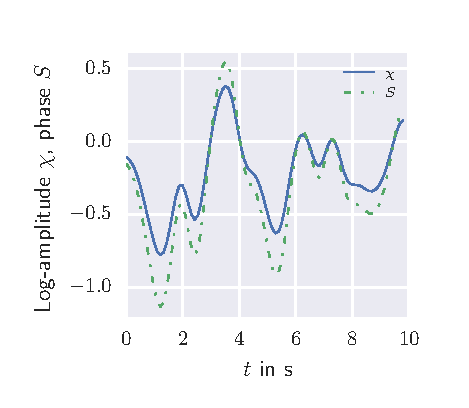
\includegraphics[]{../figures/manual/turbulence-model/logamp_and_phase}
  \caption{Amplitude and phase fluctuations as function of time. The fluctuations are less strong for the amplitude fluctuations due to saturation.}
  \label{fig:results_tone_logamp_and_phase}
\end{figure}

\begin{figure}[H]
  \centering
  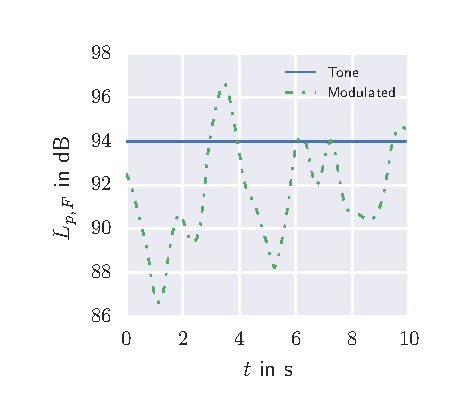
\includegraphics[]{../figures/manual/turbulence-model/modulated_levels}
  \caption{Sound pressure level of the tone as function of time, with and without fluctuations.}
  \label{fig:results_tone_levels}
\end{figure}



\begin{figure}[H]
  \centering
  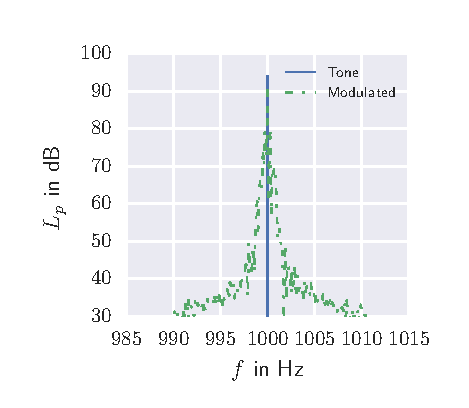
\includegraphics[]{../figures/manual/turbulence-model/tone_broadening}
  \caption{The power spectrum of the tone shows the broadening due to the phase fluctuations.}
  \label{fig:results_tone_broadening}
\end{figure}

\subsection{Scintillations as function of transverse speed}
By changing the transverse speed the refractive-index field is sampled at a
different speed. This effectively changes the correlation length and shifts the frequency range that is covered by our applied filter \cite{Wilson1999}.

Figure \ref{fig:results_scintillations_correlation} shows the correlation function for
different transverse speeds.
\begin{figure}[H]
  \centering
  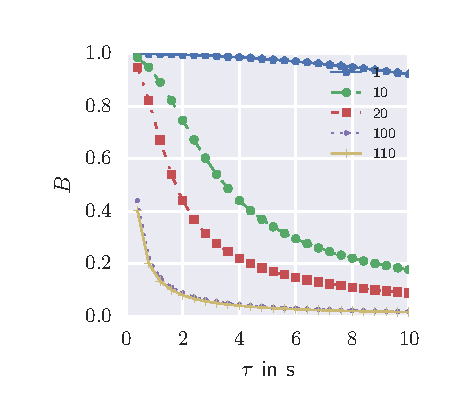
\includegraphics[]{../figures/manual/turbulence-model/correlation}
  \caption{Correlation as function of time for different transverse speeds given in meters per second.}
  \label{fig:results_scintillations_correlation}
\end{figure}
With a high transverse speed the correlation drops
faster, and this will result in relatively more high-frequency fluctuations, as is shown in Figure \ref{fig:results_scintillations_levels}.
\begin{figure}[H]
  \centering
  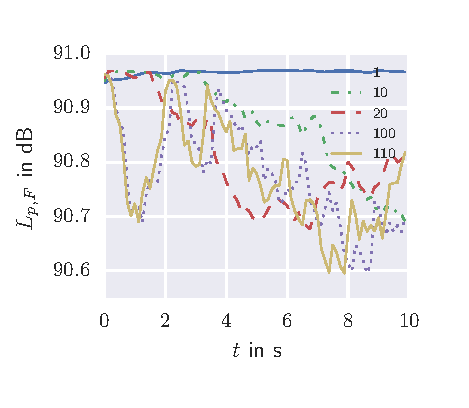
\includegraphics[]{../figures/manual/turbulence-model/scintillations_levels}
  \caption{Sound pressure level as function of time for scintillations
corresponding to different transverse speeds given in meters per second. The
same $z[n]$ were used for each case. A compression in time of the modulations with increasing velocity can be observed.}
  \label{fig:results_scintillations_levels}
\end{figure}


\subsection{Application in auralization of aircraft}
The method was developed in order to create more realistic sounding
auralizations of aircraft. An aircraft moves at high speed through the
atmosphere. A transverse speed is computed for each propagation path separately.
Because the correlation time, distance and propagation varies between the two
paths, decorrelation occurs. Figures \ref{fig:results_auralization_without} and
\ref{fig:results_auralization_with} show spectrograms respectively with and
without turbulence. The vertical lines that can be seen are the amplitude
modulations.

\begin{figure}[H]
  \centering
  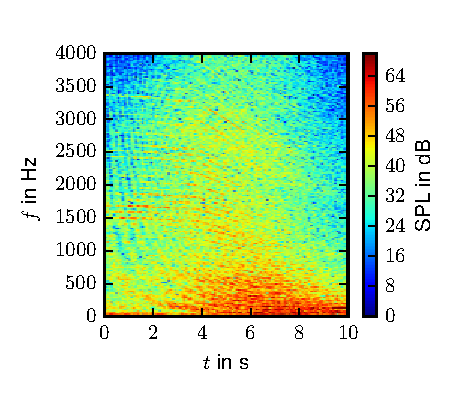
\includegraphics[]{../figures/manual/turbulence-model/auralisation_flight_without}
  \caption{Spectrogram of an auralization of an aircraft taking off.
Scintillations were not included. Visible are the ground effect and the Doppler
shift. In the initial seconds a high amount of tonal components are visible.
  }
  \label{fig:results_auralization_without}
\end{figure}

\begin{figure}[H]
  \centering
  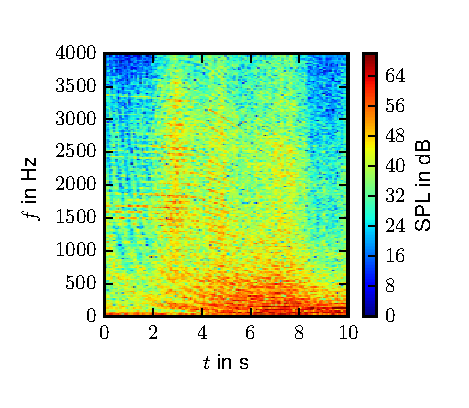
\includegraphics[]{../figures/manual/turbulence-model/auralisation_flight_both}
  \caption{Spectrogram of the same event as in Figure
  \ref{fig:results_auralization_without}, however, this time with scintillations included. Because of the high speed at which the aircraft samples the refractive-index field the scintillations are relatively high-frequent, resulting in vertical lines.}
  \label{fig:results_auralization_with}
\end{figure}

Earlier it was assumed that the correlation length was much smaller than the Fresnel zone size.
In this auralization the aircraft is moving close to the receiver. When the aircraft is closest, the distance is almost entirely given by the height which was approximately 100 meters.
The correlation length was set at 20 meters. In that case the Fresnel zone is larger than the correlation length for the lower frequencies, and equation \eqref{eq:model_daigle} is not valid.
Instead, the log-amplitude and phase variances should scale with respectively $d^3$ and $2k^2 d$ instead of $k^2 d$ \cite{Ishimaru1997}.


\subsection{Influence of parameters}

\begin{figure}[H]
%     \centering
    \begin{subfigure}{\textwidth}
        \includegraphics{{{../figures/generated/turbulence-parameters/turbulence-1.0-1e-05}}}
        \caption{\SI{1}{\meter}}
    \end{subfigure}
    ~
    \begin{subfigure}{\textwidth}
        \includegraphics{{{../figures/generated/turbulence-parameters/turbulence-10.0-1e-05}}}
        \caption{\SI{10}{\meter}}
    \end{subfigure}
    ~
    \begin{subfigure}{\textwidth}
        \includegraphics[]{{{../figures/generated/turbulence-parameters/turbulence-100.0-1e-05}}}
        \caption{\SI{100}{\meter}}
    \end{subfigure}
    \caption{The influence of the correlation length $L$.}
    \label{fig:turbulence:aircraft:parameters:correlation}
\end{figure}

\newpage
\begin{figure}[H]
%     \centering
    \begin{subfigure}{\textwidth}
        \includegraphics{{{../figures/generated/turbulence-parameters/turbulence-10.0-1e-05}}}
        \caption{\SI{1e-5}{}}
    \end{subfigure}
    ~
    \begin{subfigure}{\textwidth}
        \includegraphics{{{../figures/generated/turbulence-parameters/turbulence-10.0-1e-06}}}
        \caption{\SI{1e-6}{}}
    \end{subfigure}
    ~
    \begin{subfigure}{\textwidth}
        \includegraphics[]{{{../figures/generated/turbulence-parameters/turbulence-10.0-1e-07}}}
        \caption{\SI{1e-7}{}}
    \end{subfigure}
    \caption{The influence of the variance of the dynamic refractive-index $\sigma_{\mu}^2$.}
    \label{fig:turbulence:aircraft:parameters:variance}
\end{figure}


\section{Conclusion}
Fluctuations in the refractive-index field due to variations in temperature and
wind affects sound propagation and causes audible modulations. A method was
presented for generating sequences of modulations and applying these to
monochromatic as well as broadband signals.

A Rytov approximation to first-order refractive-index flucutuations results in a complex
phase which we can write as a log-amplitude $\chi$ and phase $S$ fluctuation.
The propagating sound is modelled as a time-varying channel where we consider
two sequences, one for the log-amplitude fluctuations, and another for the phase
fluctuations.

The fluctuations are frequency-dependent and therefore a filter was designed to take that into account.
% A Gaussian applied filter was used to model the atmospheric turbulence because of its simplicity and because it is computationally least demanding.
A Gaussian turbulence spectrum was considered, but the general method can be
used with other turbulence spectra as well. The Von Karman spectrum describes
real turbulence spectra typically better than the Gaussian spectrum, however,
the Von Karman spectrum is computationally much more demanding.
% The Gaussian model also allows implementing the phase fluctuation with a Variable Delay Line (VDL).

Examples are shown where the method is applied to a tone and to an aircraft
auralization. The aircraft auralization spectrogram shows several spikes
corresponding to amplitude modulations as well as an increase in the amount of
decorrelation. Furthermore the transverse velocity dependence on the frequency
content of the modulations is demonstrated.

According to the authors the method results in more realistic sounding
auralizations, but this has not been validated yet with listening tests. The
implementation of the model that was used in this paper to generate the figures
can be found at \cite{Rietdijk2016}.
